%% LyX 2.2.2 created this file.  For more info, see http://www.lyx.org/.
%% Do not edit unless you really know what you are doing.
\documentclass[english,a4paper]{article}
\usepackage[T1]{fontenc}
\usepackage[latin9]{inputenc}
\usepackage{geometry}
\geometry{verbose,tmargin=1.5cm,bmargin=1.5cm,lmargin=2cm,rmargin=2cm}
\pagestyle{empty}
\usepackage{float}
\usepackage{amsmath}
\usepackage{graphicx}
\usepackage{wasysym}

\makeatletter

%%%%%%%%%%%%%%%%%%%%%%%%%%%%%% LyX specific LaTeX commands.
%% Because html converters don't know tabularnewline
\providecommand{\tabularnewline}{\\}
\floatstyle{ruled}
\newfloat{algorithm}{tbp}{loa}
\providecommand{\algorithmname}{Algorithm}
\floatname{algorithm}{\protect\algorithmname}

\makeatother

\usepackage{babel}
\usepackage{listings}
\renewcommand{\lstlistingname}{Listing}

\begin{document}

\title{2ID90 International Draught assignment}

\author{Group 19: Daan de Graaf, Yoeri Poels}
\maketitle

\section{Introduction}

\emph{Give a short introduction on your project: state the objectives
and comment on how they are achieved. Further more, in the whole document,
please take care of the following:}
\begin{itemize}
\item \emph{Refer to any material you used to obtain your results}, e.g.
\cite{Ertel:2011:IAI:1971988}\emph{.}
\item \emph{Illustrate your material with appropriate figures which are
numbered and have a descriptive caption. Refer to the figure in the
text: see }Figure \ref{fig:The-winners}\emph{.}
\begin{figure}[bh]
\begin{centering}
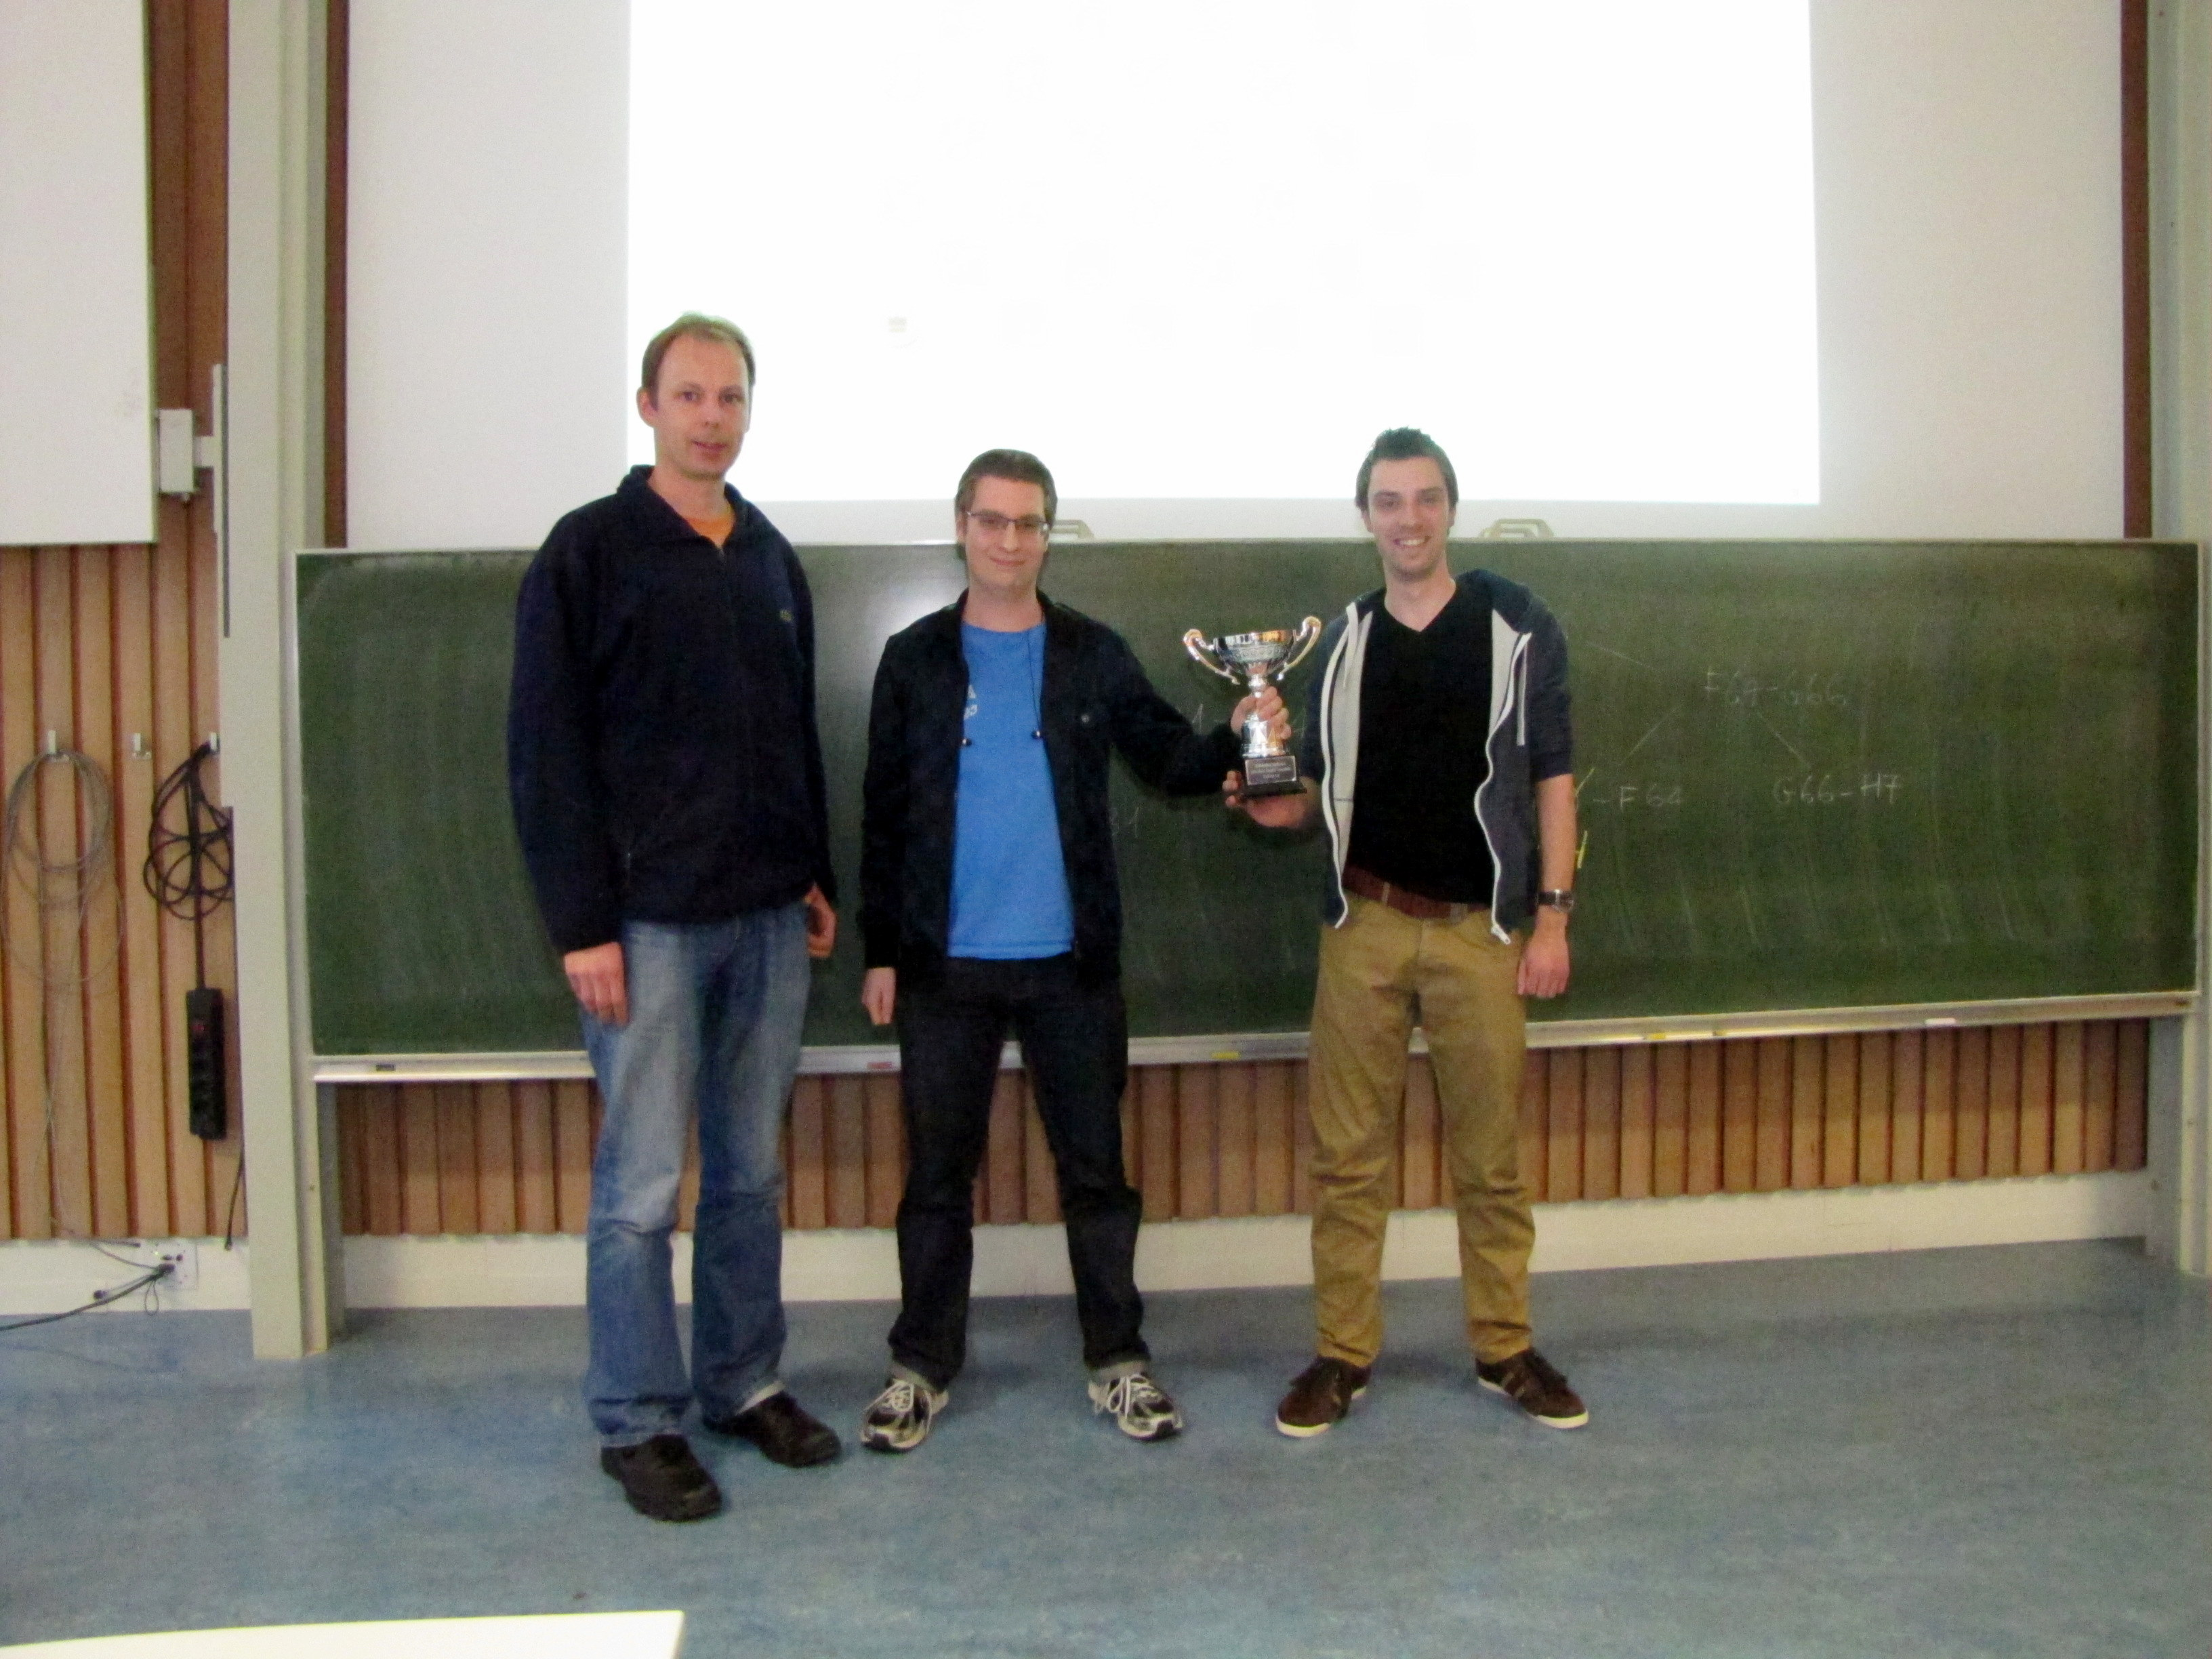
\includegraphics[scale=0.07]{IMG_7778.JPG}
\par\end{centering}
\emph{\caption{\label{fig:The-winners}The winners of the 2ID90 international draughts
tournament, edition 2014.}
}

\end{figure}
\item \emph{Use pseudo-code to explain your algorithms. Note that pseudo-code
is not the same as your actual java code. It should be an abstraction
of that code and should be presented with readability and clarity
in mind. Pseudo-code has to be accompanied with proper explanation
and argumentation.}
\item \emph{Use numbered mathematical formulas instead of lengthy explanations
in text. Additionally, discuss the principles behind the formula.}
\end{itemize}

\section{Alpha-Beta }

We made the decision early on to implement alpha-beta pruning in the single method below, in contrast to having two separate methods that are very similar in an effort to reduce code duplication. We added an extra boolean parameter 'maximize' to indicate whether the algorithm should minimize or maximize the evaluation function. 
We also added a 'depth' parameter to indicate how deep down the tree the algorithm may search. Upon a recursive call the 'maximize' parameter is flipped, and the 'depth' is decreased by 1. If the method is called with depth 0, the heuristic evaluation of the node is returned. 
We have added one more parameter 'didCapture', which is set to true only if the method was called recursively and in the given node state the previous move was a capture. This is only used to make sure that the best move of node is not set to a move that occurs after a capture, as captures do not count towards the depth. 
On top of this we also extend the search depth by two layers if the depth reaches 0 on a node that is not quiet.
The resulting algorithm then becomes:

\begin{algorithm}[h]
\begin{lstlisting}[language=Java,numbers=left,numberstyle={\footnotesize},stepnumber=2,basicstyle={\scriptsize},tabsize=4, mathescape=true]
int AlphaBeta(node, alpha, beta, depth, maximize, didCapture) {
	// Search up to two extra nodes further if the current node is not quiet
	if ((depth <= 0 && isQuiet(node)) || depth <= -2)	 { return Evaluate(node); }
	int bestValue = maximize ? $\infty$ : $-\infty$;
	
	for (move : PossibleMoves(node) {
		node.doMove(move);	// Apply this move so we can evaluate the state
		int newDepth;
		if (move.isCapture()) {
			newDepth = depth; // Do not count captures in the search depth	
		} else {
			newDepth = depth - 1;
		}
	
		int value = AlphaBeta(node, alpha, beta, newDepth, !maximize, m.isCapture());
		if (maximize && value >= bestValue) {
			bestValue = value;
			if (depth == searchDepth && !didCapture) {
				// We are at the root of the search tree
				node.setBestMove(move);				
			}
			
			if (bestValue >= beta) {
				node.undoMove(move); // Undo move for clean return
				return bestValue;
			}
		}
		else if (!maximize && value <= bestValue) {
			bestValue = value;
			if (depth == searchDepth && !didCapture) {
				node.setBestMove(move);			
			}
			
			if (bestValue <= alpha) {
				node.undoMove(move);
				return bestValue;			
			}
		}
		node.undoMove(move); // Undo the move so we can reuse the node for the next iteration of the loop		
	}
	return bestValue;
	
}
\end{lstlisting}

\caption{\label{alg:AlphaBeta}AlphaBeta}
\end{algorithm}


\section{Iterative Deepening}

We implement iterative deepening by first running Algorithm \ref{alg:AlphaBeta} with an initial search depth 'baseSearchDepth' and storing this move. Then while we still have time we keep repeating this process with an increasing search depth until the time runs out. When the time runs out the alphaBeta method throws an AIStoppedException, which is caught here and  The algorithm is given by:

\begin{algorithm}[h]
\begin{lstlisting}[language=Java,numbers=left,numberstyle={\footnotesize},stepnumber=2,basicstyle={\scriptsize},tabsize=4, mathescape=true]
Move IterativeDeepening(State s) {
        bestMove = null;
        try {
            node = new Node(s.clone());
            
            // Set to initial search depth
            searchDepth = baseSearchDepth;
            // Loop while not interrupted
            while (true) {
                bestValue = alphaBeta(node, $-\infty$, $\infty$, searchDepth, s.isWhiteToMove(), false);
                bestMove = node.getBestMove();
                if ((bestValue == MAX_VALUE && s.isWhiteToMove())
                        || (bestValue == MIN_VALUE && !s.isWhiteToMove())) {
                    // We have a winning strategy
                    break;
                }

                searchDepth++; // Increase the search depth for the next iteration
            }

        } catch (AIStoppedException ex) {
        		// Our time is up, return the best move according to the highest search depth reached
	        	return bestMove;
        }
}
\end{lstlisting}

\caption{\label{alg:Iterative}IterativeDeepening}
\end{algorithm}


\section{Evaluation}

Our evaluation of board state \emph{s} is split up in several parts, with each having a different weight. The total evaluation-score is based on an evaluation of the \textbf{amount of pieces and kings}, the \textbf{tempi}, \textbf{balance} and \textbf{coherence} of both sides, and the amount of moves that can be made. \\ \\
The score for the amount of pieces/kings \emph{piecesScore} is calculated in the following way:
\begin{equation}
piecesScore(s) = (\fullmoon(s) + 3 \cdot \fullmoon king(s)) - (\newmoon(s) + 3 \cdot \newmoon king(s))
\end{equation}
where for board state \emph{s}, \fullmoon(s) and \newmoon(s) are the number of white and black pieces, and \fullmoon king(s) and \newmoon king(s) are the number of white and black kings, respectively.\\ We use this to evaluate since having more pieces / the opponents losing pieces means you are more likely to win, as you lose when you do not have any pieces left. \\ \\
The score for the tempi of both sides \emph{tempiScore} is calculated in the following way: 
\begin{equation}
tempiScore(s) = whiteTempi(s) - blackTempi(s) \\
\end{equation}
where \emph{whiteTempi} and \emph{blackTempi} are the following:\\
\begin{algorithm}[h]
	\begin{lstlisting}[language=Java,numbers=left,numberstyle={\footnotesize},stepnumber=2,basicstyle={\scriptsize},tabsize=4]
	int whiteTempi(State s) {
		whiteTempi = 0;
		for (every white piece in state s) 
			whiteTempi = whiteTempi + distance from white piece to bottom row (in number of rows);
		}
		return whiteTempi;
	}
	
	int blackTempi(State s) {
		blackTempi = 0;
		for (every black piece in state s) 
			blackTempi = blackTempi + distance from black piece to top row (in number of rows);
		}
		return blackTempi;
	}
	\end{lstlisting}
\end{algorithm} \\
An example of whiteTempi (total value being 23) is shown in Figure \ref{fig:WhiteTempi}: 
\begin{figure}[bh]
	\begin{centering}
		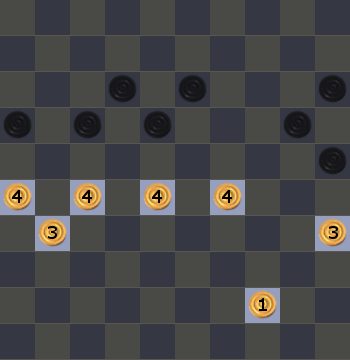
\includegraphics[scale=0.35]{tempi_white.png}
		\par\end{centering}
	\emph{\caption{\label{fig:WhiteTempi}An example of whiteTempi}
	}
\end{figure}


	Give a clear explanation of your evaluation function. Compare
alternative evaluation strategies, alternative parameter settings,
etcetera. Argue why you have chosen a particular evaluation function:
make measurements and use graphs and tables where necessary. Use formulas
(like (\ref{eq:Hs})\emph{) or pseudo-code:
\begin{equation}
H(s)=\begin{cases}
\infty & \fullmoon(s)=0\\
-\infty & \newmoon(s)=0\\
\fullmoon(s)-\newmoon(s) & otherwise
\end{cases},\label{eq:Hs}
\end{equation}
where for board state $s$, $\fullmoon(s)$ and $\newmoon(s)$ are
the number of white and black pieces, respectivily.}

\section{Custom extensions}

We have handled quiescence in Algorithm \ref{alg:AlphaBeta}, where at depth 0 we also check if the board state is currently quiet. If it is we return the heuristic evaluation of the node, otherwise we allow the search to continue up to 2 levels further in the tree. to check if a state is quiet we use the following simple algorithm:

\begin{algorithm}[h]
\begin{lstlisting}[language=Java,numbers=left,numberstyle={\footnotesize},stepnumber=2,basicstyle={\scriptsize},tabsize=4, mathescape=true]
Move IsQuiet(State s) {
        moves = s.getMoves();
        if (moves.isEmpty()) {
        		// No pieces are left on the board
        		return true;
        	}
        return !moves.get(0).isCapture();
}
\end{lstlisting}

\caption{\label{alg:Iterative}IsQuiet}
\end{algorithm}

We also ignore obliged moves in the search depth, as can be seen on line 9-10 of Algorithm. \ref{alg:AlphaBeta}.

These extensions did make the AI stronger, but only slightly. When an otherwise identical version without these modifications (A) plays against the version with these extensions (B), A will draw B when A is white. But when B is white, it will win by a slight edge it has with the extensions. This is most visible in the end game:

\begin{figure}[bh]
	\begin{centering}
		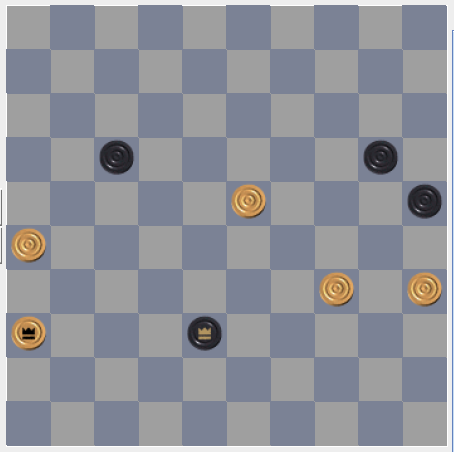
\includegraphics[scale=0.35]{extensions1.png}
		\par\end{centering}
	\emph{\caption{The game is nearly tied in piece count and the two kings suggest a draw outcome}
	}
\end{figure}

\begin{figure}[bh]
	\begin{centering}
		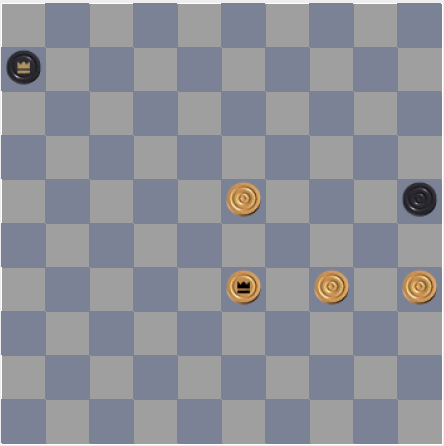
\includegraphics[scale=0.35]{extensions2.png}
		\par\end{centering}
	\emph{\caption{A is to move and has to strike the king and another piece, allowing B to capture the king and force A to put its last piece in harms way.}
	}
\end{figure}

\begin{figure}[bh]
	\begin{centering}
		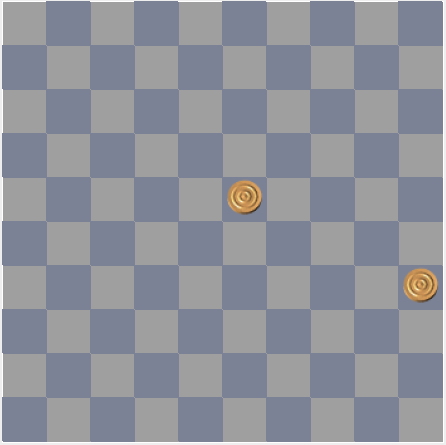
\includegraphics[scale=0.35]{extensions.png}
		\par\end{centering}
	\emph{\caption{B wins by exploring further}
	}
\end{figure}

\section{Results}

\emph{If you did not do so already in the previous sections, you can
show your final results here. Again you can use graphs and tables
to show your point.}

\section{Conclusions}

\emph{A short logical summing up of the main reported results.}

\section{Contributions}

\emph{A statement on the contributions of each of the authors.}

\begin{tabular}{|c|c|c|c|}
\cline{2-4} 
\multicolumn{1}{c|}{} & \textbf{implementation} & \textbf{documentation} & \textbf{total \#hours}\tabularnewline
\hline 
Author 1 & 60\% & 30\% & 30\tabularnewline
\hline 
Author 2 & 40\% & 70\% & 25\tabularnewline
\hline 
\end{tabular}
\begin{itemize}
\item \emph{At least the given columns in the table need to be filled in,
add columns if needed.}
\item \emph{Add comments to clarify your table entries when necessary.}
\item \emph{...}
\end{itemize}
\bibliographystyle{plain}
\bibliography{references}

\end{document}
